\documentclass{beamer}

% --- Theme ---
\usetheme{metropolis} % Use a clean, modern theme. If metropolis is not available, default or Madrid are fallback options.
\usecolortheme{default}
\setbeamercolor{background canvas}{bg=white}

% --- Packages ---
\usepackage[utf8]{inputenc}
\usepackage[T1]{fontenc}
\usepackage{graphicx}
\usepackage{amsmath,amssymb,amsfonts}
\usepackage{booktabs}
\usepackage{multirow}
\usepackage{hyperref}
\usepackage{tikz}
\usetikzlibrary{calc,positioning,shapes.geometric,arrows.meta,3d,shadows}

% --- Metadata ---
\title{DisaggKV: Scalable and Disaggregated CXL-PIM Pooling for Multi-Tenant LLM Serving}
\subtitle{Rearchitecting Multi-Tenant LLM Serving Interconnects}
\author{Kaichen Li}
\institute{Department of Computer and Information Engineering \\ Youngsan University, South Korea}
\date{\today}

\begin{document}

% 1. Title Slide
\begin{frame}
    \titlepage
\end{frame}

% 2. Introduction & Motivation
\begin{frame}{Introduction: The LLM Memory Challenge}
    \begin{itemize}
        \item \textbf{Explosive Demand}: Multi-tenant LLM serving pushes infrastructures to limits.
        \item \textbf{KV Cache Footprint}: 7B model @ 128K context consumes \textbf{>7GB} per request.
        \item \textbf{HBM Exhaustion}: Local GPU HBM is rapidly exhausted by concurrent batches.
        \item \textbf{CXL Solution}: Enables physical memory pooling, but introduces performance degradation during autoregressive decoding.
    \end{itemize}
\end{frame}

\begin{frame}{Motivation: The Throughput Bottleneck}
    \begin{itemize}
        \item \textbf{Host-Aggregated CXL}: Standard CXL 2.0 pools rely on Host to fetch all data.
        \item \textbf{Data Movement}: Fetching dense KV vectors across Host-indirected CXL fabric saturates PCIe bandwidth.
        \item \textbf{SLA Violation}: Violates strict 99\% tail-latency (e.g., 50ms) Service-Level Agreements.
    \end{itemize}
    \vspace{0.5cm}
    \begin{block}{The Problem}
        Repeatedly fetching dense historical KV vectors to resolve Attention dot-products creates a severe I/O congestion wall.
    \end{block}
\end{frame}

% 3. Problem Statement (Queuing Theory)
\begin{frame}{The Queue Congestion Wall: M/D/1 Theory}
    \begin{itemize}
        \item Expected delay $W_q$ in a deterministic network port:
        \[ W_q = \frac{\rho}{2\mu(1 - \rho)} \quad \text{where} \quad \rho = \frac{\lambda}{\mu} \]
        \item \textbf{$\lambda$ (Arrival rate)}: Increases with distributed KV subsets.
        \item \textbf{$\mu$ (Service rate)}: Restricted by PCIe Gen6 x16 (64GB/s).
        \item As $\rho \to 1$, queue latency grows asymptotically.
    \end{itemize}
    \vspace{0.2cm}
    \centering
    \textit{Strategy: Suppress arrival density $\lambda$ at the central node by keeping computation co-located at endpoints.}
\end{frame}

% 4. DisaggKV Architecture
\begin{frame}{DisaggKV: System Overview}
    \centering
    \resizebox{0.75\textwidth}{!}{
    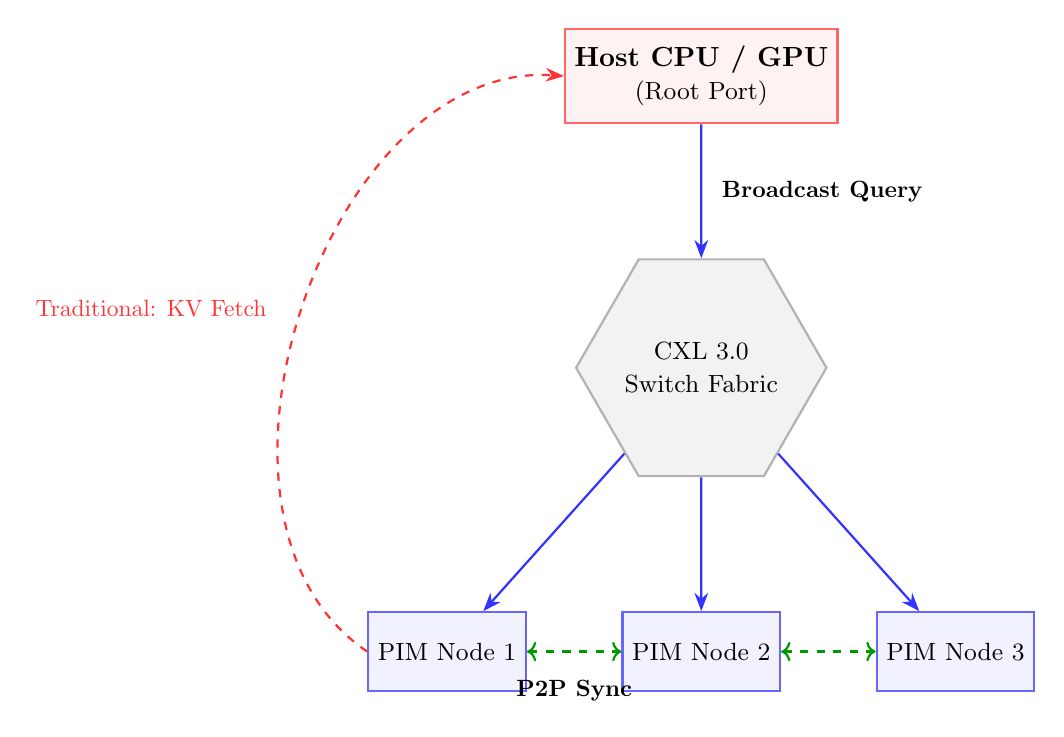
\begin{tikzpicture}[
        node distance=1.1cm,
        host/.style={rectangle, draw=red!60, fill=red!5, thick, minimum width=3.0cm, minimum height=1.2cm, align=center},
        switch/.style={regular polygon, regular polygon sides=6, draw=gray!60, fill=gray!10, thick, minimum size=2.5cm, inner sep=0pt, align=center},
        node/.style={rectangle, draw=blue!60, fill=blue!5, thick, minimum width=2.0cm, minimum height=1.0cm, align=center},
        arrow/.style={thick, -Stealth}
    ]
        % Nodes
        \node (host) [host] {\textbf{Host CPU / GPU}\\\small (Root Port)};
        \node (switch) [switch, below=1.7cm of host] {\small CXL 3.0\\\small Switch Fabric};
        
        \node (n2) [node, below=1.7cm of switch] {\small PIM Node 2};
        \node (n1) [node, left=1.2cm of n2] {\small PIM Node 1};
        \node (n3) [node, right=1.2cm of n2] {\small PIM Node 3};
    
        % High-level Traffic
        \draw [arrow, dashed, red!80, bend left=75] (n1.west) to node[midway, left=0.35cm, scale=0.85] {Traditional: KV Fetch} (host.west);
        
        \draw [arrow, draw=blue!80] (host) -- (switch) node[midway, right=0.15cm, scale=0.85] {\textbf{Broadcast Query}};
        \draw [arrow, draw=blue!80] (switch) -- (n1);
        \draw [arrow, draw=blue!80] (switch) -- (n2);
        \draw [arrow, draw=blue!80] (switch) -- (n3);
        
        \draw [arrow, <->, draw=green!60!black, dashed] (n1) -- (n2) node[midway, below=0.25cm, scale=0.85] {\textbf{P2P Sync}};
        \draw [arrow, <->, draw=green!60!black, dashed] (n2) -- (n3);
    \end{tikzpicture}
    }
    \caption{Transforming interconnect from congested data-fetch bus into reduction fabric.}
\end{frame}

\begin{frame}{Core Contribution 1: Locality-Aware Paging}
    \begin{itemize}
        \item \textbf{Segregation}: Shared Hot Pages (e.g., System Prompts) vs. Private Contexts.
        \item \textbf{Pinned Prompts}: High-contention prompts pinned to dedicated CXL nodes.
        \item \textbf{Dynamic Migration}: Monitor CXL switch queue depths; migrate blocks to idle nodes to ensure balanced load ($\rho$).
        \item \textbf{Benefit}: Prevents redundant read amplification and balances bandwidth.
    \end{itemize}
\end{frame}

\begin{frame}{Core Contribution 2: Fabric Distributed Reduction}
    \begin{itemize}
        \item \textbf{P2P Synchronization}: Two-Phase Commit communicating via switch-level P2P links.
        \item \textbf{Process}:
            \begin{enumerate}
                \item Local assessment of maximum logit (\texttt{PIM\_SEND\_PARTIAL}).
                \item Global Max Distribution asynchronously.
                \item Global Summation accumulation.
            \end{enumerate}
        \item \textbf{Effect}: Exchanging kilobytes of scalars instead of gigabytes of matrices.
        \item \textbf{Resiliency}: Async FIFOs absorb fabric jitter and random delays.
    \end{itemize}
\end{frame}

% 5. Evaluation Results
\begin{frame}{Evaluation: Throughput & SLA Compliance}
    \centering
    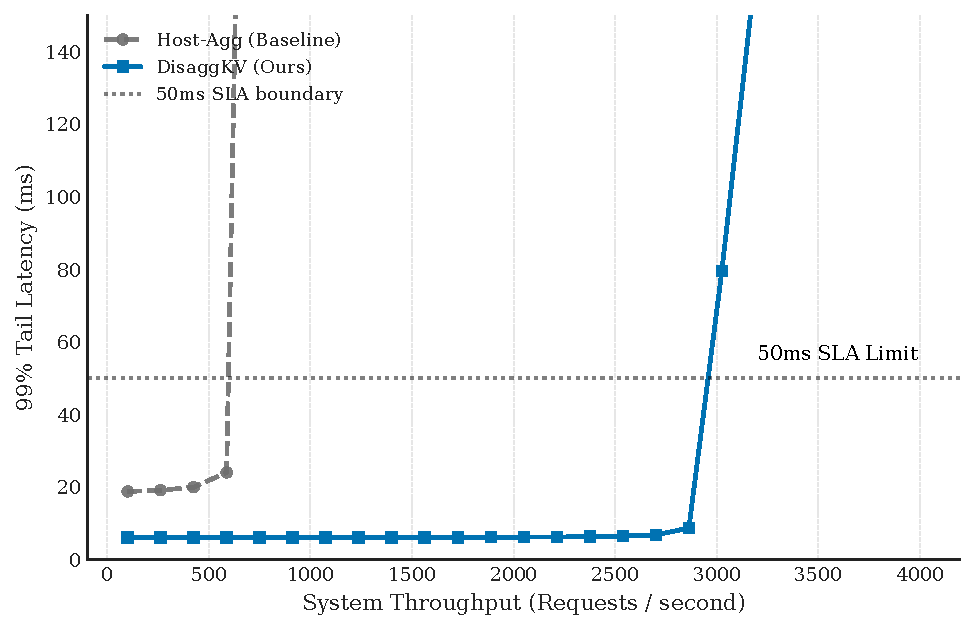
\includegraphics[width=0.7\textwidth]{paper_assets/figures/fig1_throughput_latency.pdf}
    \begin{itemize}
        \item DisaggKV maintains stable tail latency (\textbf{<15ms}) up to 3000 req/s.
        \item Host-Aggregated violates 50ms SLA at 600 req/s.
        \item \textbf{5x Throughput Improvement}.
    \end{itemize}
\end{frame}

\begin{frame}{Evaluation: Topology Scalability}
    \centering
    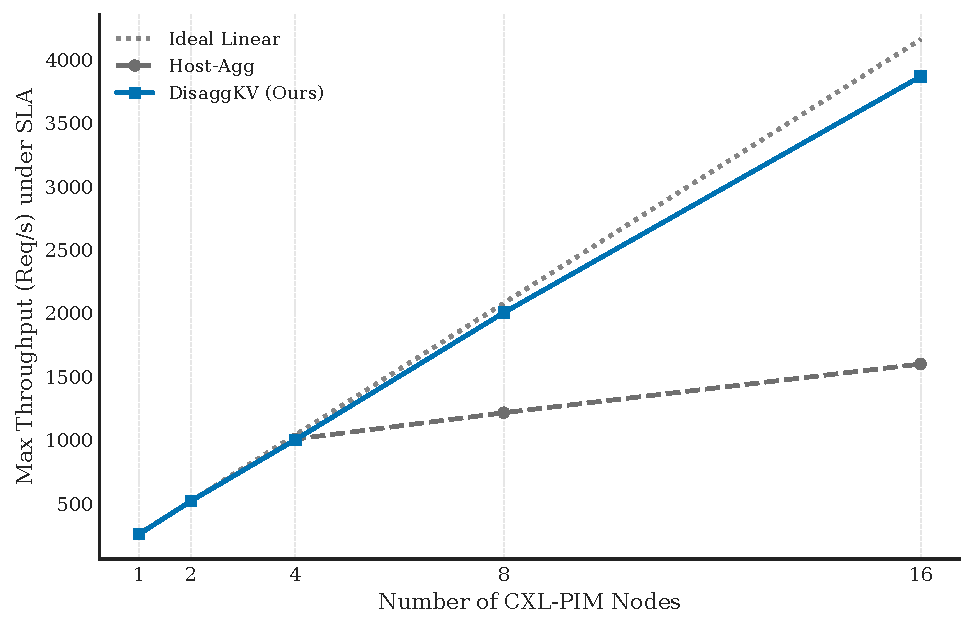
\includegraphics[width=0.7\textwidth]{paper_assets/figures/fig2_scalability.pdf}
    \begin{itemize}
        \item \textbf{Near-Linear Scaling}: Near-ideal horizontal expansion up to 8 nodes.
        \item Host-Aggregated yields diminishing returns due to Root Complex port contention.
    \end{itemize}
\end{frame}

\begin{frame}{Evaluation: Bandwidth Reduction}
    \centering
    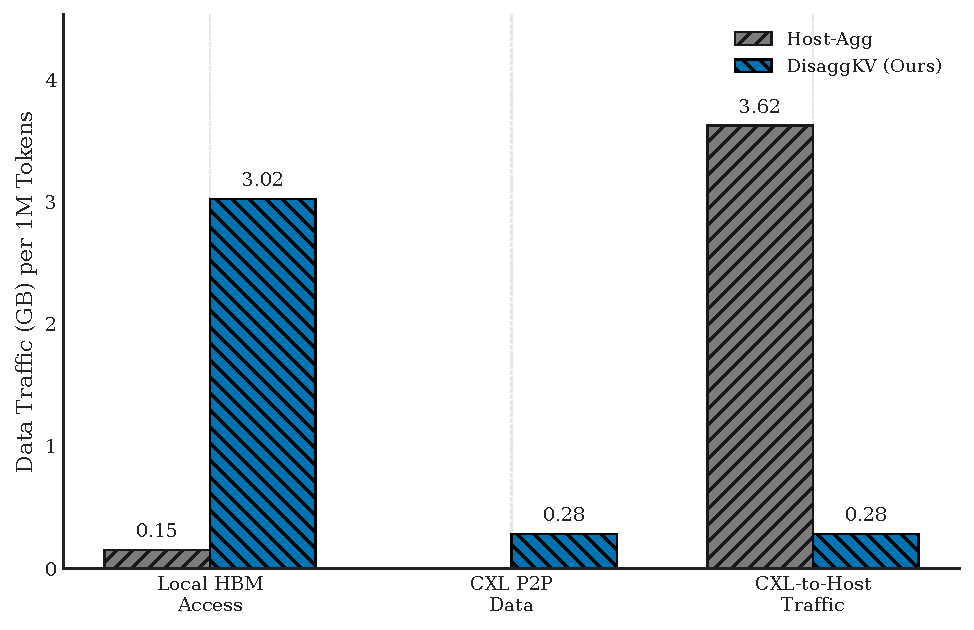
\includegraphics[width=0.7\textwidth]{paper_assets/figures/fig3_network_breakdown.pdf}
    \begin{itemize}
        \item Global switch traffic reduced by over \textbf{92\%}.
        \item Replaces dense matrix transfers with condensed scalar operations.
    \end{itemize}
\end{frame}

\begin{frame}{Evaluation: Fault Recovery & Sensitivity}
    \begin{columns}
        \begin{column}{0.5\textwidth}
            \centering
            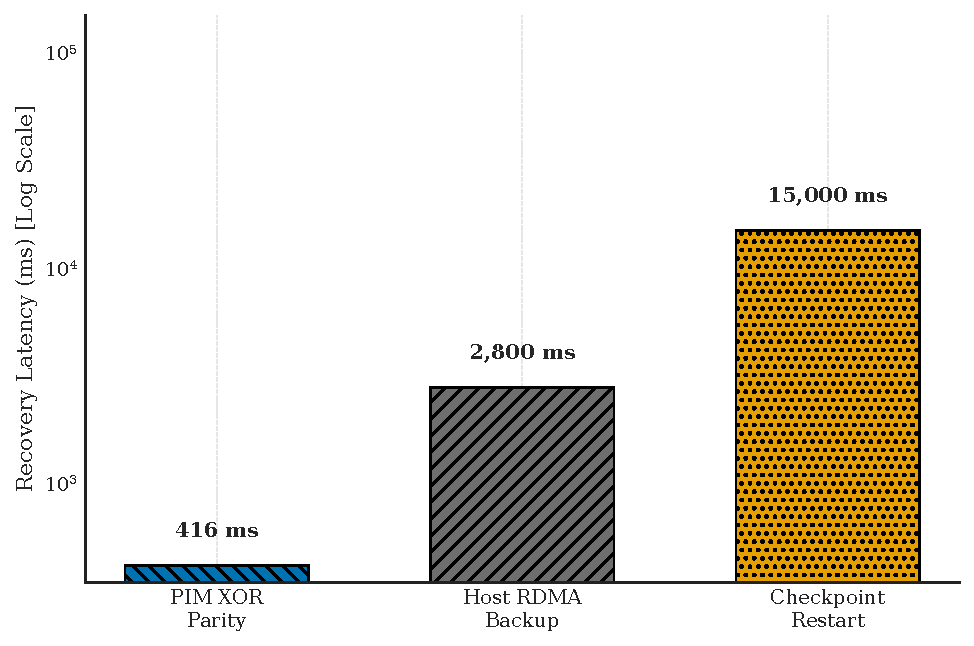
\includegraphics[width=\textwidth]{paper_assets/figures/fig4_fault_recovery.pdf}
            \small Sub-second restoration (P99 < 500ms).
        \end{column}
        \begin{column}{0.5\textwidth}
            \centering
            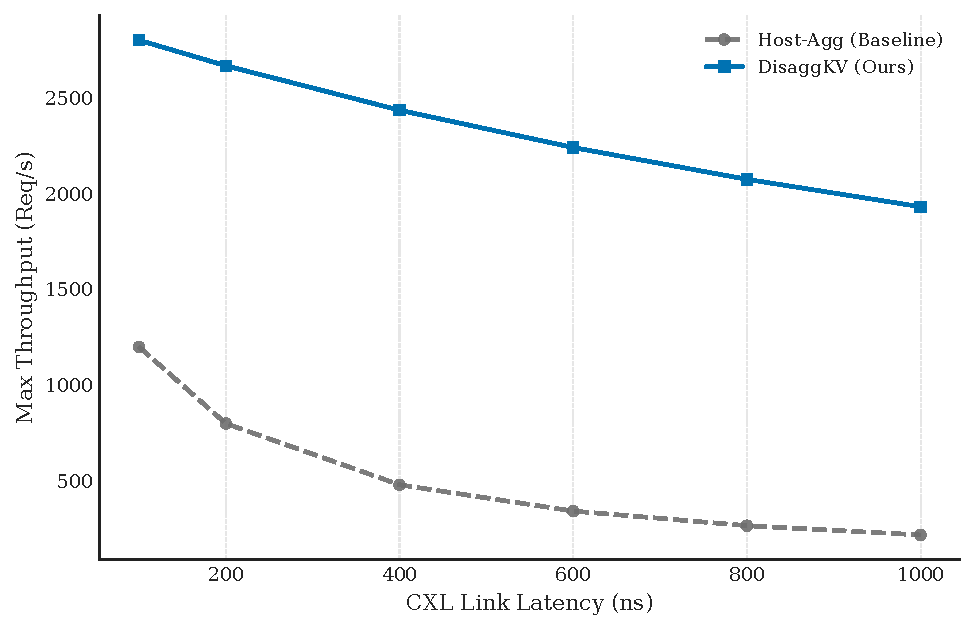
\includegraphics[width=\textwidth]{paper_assets/figures/fig5_sensitivity_latency.pdf}
            \small Resilient to network diameter/latency increase.
        \end{column}
    \end{columns}
    \vspace{0.3cm}
    \begin{itemize}
        \item PIM-side XOR parity recovery vs. multi-second Host software restarts.
        \item Resilient to large-scale data center cable lengths/hops.
    \end{itemize}
\end{frame}

% 6. Conclusion
\begin{frame}{Conclusion}
    \begin{itemize}
        \item \textbf{Capacity vs. Bandwidth}: DisaggKV solves the bottleneck in clustered CXL environments.
        \item \textbf{Hardware-Software Co-Design}: Hypervisor paging policy + CXL 3.0 P2P fabric.
        \item \textbf{Key Outcomes}:
            \begin{itemize}
                \item 92\% reduction in global switch traffic.
                \item 5x throughput gain under strict SLA.
                \item Sub-second fault recovery.
            \end{itemize}
        \item \textbf{Conclusion}: Critical enabler for large-scale multi-tenant LLM serving.
    \end{itemize}
    \vspace{0.5cm}
    \centering
    \textbf{\Large Thank You!} \\
    \small Questions?
\end{frame}

\end{document}
